%%%%(c)
%%%%(c)  This file is a portion of the source for the textbook
%%%%(c)
%%%%(c)    Abstract Algebra: Theory and Applications
%%%%(c)    Copyright 1997 by Thomas W. Judson
%%%%(c)
%%%%(c)  See the file COPYING.txt for copying conditions
%%%%(c)
%%%%(c)
\chap{Matrix Groups and Symmetry}{matrix}

When Felix Klein\index{Klein, Felix} (1849--1925) accepted a chair at
the University of Erlangen, he outlined in his inaugural address a
program to classify different geometries. Central to Klein's
program was the theory of groups: he considered geometry to be the
study of properties that are left invariant under transformation
groups. Groups, especially matrix groups, have now become important in
the study of symmetry and have found applications in such disciplines
as chemistry and physics. In the first part of this chapter, we will
examine some of the classical matrix groups, such as the general linear
group, the special linear group, and the orthogonal group. We will
then use these matrix groups to investigate some of the ideas behind
geometric symmetry.  


\section{Matrix Groups}

\subsection*{Some Facts from Linear Algebra}
 
Before we study matrix groups, we must recall some basic facts from
linear algebra.  One of the most fundamental ideas of linear algebra
is that of a linear transformation. A {\bfi linear
transformation\/}\index{Linear transformation!definition of} or {\bfi 
linear map}\index{Linear map} $T : {\Bbb R}^n \rightarrow {\Bbb R}^m$
is a map that preserves vector addition and scalar multiplication;
that is, for vectors ${\bold x}$ and ${\bold y}$ in ${\Bbb R}^n$ and a
scalar $\alpha \in {\Bbb R}$, 
\begin{eqnarray*}
T({\bold x}+{\bold y}) & = & T({\bold x}) + T({\bold y}) \\
T(\alpha {\bold y}) & = & \alpha T({\bold y}).
\end{eqnarray*}
An $m \times n$ matrix with entries in ${\Bbb R}$ represents a linear
transformation from ${\Bbb R}^n$ to ${\Bbb R}^m$. If we write vectors
${\bold x} = (x_1, \ldots, x_n)^{\rm t}$ and ${\bold y} = (y_1,
\ldots, y_n)^{\rm t}$ in ${\Bbb R}^n$ as column matrices, then an $m
\times n$ matrix 
\[
A
=
\left(
\begin{array}{cccc}
a_{11} & a_{12} & \cdots & a_{1n} \\
a_{21} & a_{22} & \cdots & a_{2n} \\
\vdots & \vdots & \ddots & \vdots \\
a_{m1} & a_{m2} & \cdots & a_{mn}
\end{array}
\right)
\]
maps the vectors to ${\Bbb R}^m$ linearly by matrix
multiplication.  Observe that if $\alpha$ is a real number,
\begin{eqnarray*}
A({\bold x} + {\bold y} ) 
& = & 
A {\bold x }+ A {\bold y} \\
\alpha A {\bold x} 
& = & 
A ( \alpha {\bold x}),
\end{eqnarray*}
where
\[
{\bold x}
=
\left(
\begin{array}{c}
x_1 \\
x_2 \\
\vdots \\
x_n
\end{array}
\right).
\]
We will often abbreviate the matrix $A$ by writing
$(a_{ij})$\label{matrixnote}.  
 
 
Conversely, if $T : {\Bbb R}^n \rightarrow {\Bbb R}^m$ is a linear
map, we can associate a matrix $A$ with $T$ by considering what $T$
does to the vectors 
\begin{eqnarray*}
{\bold e}_1 & = & (1, 0, \ldots, 0)^{\rm t} \\
{\bold e}_2 & = & (0, 1, \ldots, 0)^{\rm t} \\
            &  \vdots &  \\
{\bold e}_n & = & (0, 0, \ldots, 1)^{\rm t}.
\end{eqnarray*}
We can write any vector ${\bold x} = (x_1, \ldots, x_n)^{\rm t}$ as
\[
x_1 {\bold e}_1 + x_2 {\bold e}_2 + \cdots + x_n {\bold e}_n.
\]
Consequently, if
\begin{eqnarray*}
T({\bold e}_1) & = & (a_{11}, a_{21}, \ldots, a_{m1})^{\rm t}, \\
T({\bold e}_2) & = & (a_{12}, a_{22}, \ldots, a_{m2})^{\rm t}, \\
            &  \vdots &  \\
T({\bold e}_n) & = & (a_{1n}, a_{2n}, \ldots, a_{mn})^{\rm t},
\end{eqnarray*}
then
\begin{eqnarray*}
T({\bold x} )
& = &
T(x_1 {\bold e}_1 + x_2 {\bold e}_2 + \cdots + x_n {\bold e}_n) \\
& = &
x_1 T({\bold e}_1) + x_2 T({\bold e}_2) + \cdots + x_n T({\bold e}_n)
\\ 
& = &
\left( \sum_{k=1}^{n} a_{1k} x_k, \ldots,  \sum_{k=1}^{n} a_{mk} x_k
\right)^{\rm t} \\ 
& = & 
A {\bold x}.
\end{eqnarray*}
 
 
\begin{example}{linear_transform}
If we let $T : {\Bbb R}^2 \rightarrow {\Bbb R}^2$ be the map given by 
\[
T(x_1, x_2) = (2 x_1 + 5 x_2, - 4 x_1 + 3 x_2),
\]
the axioms that $T$ must satisfy to be a linear transformation are
easily verified. The column vectors $T {\bold e}_1 = (2, -4)^{\rm t}$
and $T {\bold e}_2 = (5,3)^{\rm t}$  tell us that $T$ is given by the
matrix 
\[
A =
\left(
\begin{array}{cc}
2 & 5 \\
-4 & 3
\end{array}
\right).
\]
\end{example}
 
 
Since we are interested in groups of matrices, we need to know
which matrices have multiplicative inverses. Recall that an $n \times
n$ matrix $A$ is {\bfi invertible\/}\index{Matrix!invertible} exactly
when there exists another matrix $A^{-1}$ such that $A A^{-1} = A^{-1}
A = I$, where 
\[
I =
\left(
\begin{array}{cccc}
1 & 0 & \cdots & 0 \\
0 & 1 & \cdots & 0 \\
\vdots & \vdots & \ddots & \vdots \\
0 & 0 & \cdots & 1
\end{array}
\right)
\]
is the $n \times n$ identity matrix. From linear algebra we know that
$A$ is invertible if and only if the determinant of $A$ is nonzero.
Sometimes an invertible matrix is said to be {\bfi
nonsingular}\index{Matrix!nonsingular}. 
 
 
\begin{example}{inverse_matrix}
If $A$ is the matrix
\[
\left(
\begin{array}{cc}
2 & 1 \\
5 & 3
\end{array}
\right),
\]
then the inverse of $A$ is
\[
A^{-1} =
\left(
\begin{array}{cc}
3 & -1 \\
-5 & 2
\end{array}
\right).
\]
We are guaranteed  that $A^{-1}$ exists, since $\det(A) = 2 \cdot 3 - 5
\cdot 1 = 1$ is nonzero. \mbox{\hspace*{1in}}
\end{example}
 
 
Some other facts about determinants will also prove useful in the
course of this chapter.   Let $A$ and $B$ be $n \times n$ matrices.
From linear algebra we have the following properties of determinants.
\begin{itemize}
 
\item
The determinant is a homomorphism into the multiplicative group of
real numbers; that is, $\det( A B) = (\det A )(\det B)$. 
 
\item
If $A$ is an invertible matrix, then $\det(A^{-1}) = 1 / \det A$.
 
\item
If we define the transpose  of a matrix $A = (a_{ij})$ to be $A^{\rm
t} = (a_{ji})$, then $\det(A^{\rm t}) = \det A$. 
 
\item
Let $T$ be the linear transformation associated with an $n \times n$
matrix $A$. Then $T$ multiplies volumes by a factor of $|\det A|$. In
the case of ${\Bbb R}^2$, this means that $T$ multiplies areas by
$|\det A|$.
 
\end{itemize}
 
 
Linear maps, matrices, and determinants are covered in any elementary
linear algebra text; however, if you have not had a course in linear
algebra, it is a straightforward process to verify these properties
directly for $2 \times 2$ matrices, the case with which we are most
concerned. 
 
 
 
\subsection*{The General and Special Linear Groups}
 
The set of all $n \times n$  invertible matrices forms a group called
the {\bfi general linear group}\index{Group!general linear}.  We will
denote this group by $GL_n({\Bbb R})$.  The general linear group has
several important subgroups. The multiplicative properties of the
determinant imply that the set of matrices with determinant one is a
subgroup of the general linear group.  Stated another way, suppose
that $\det(A) =1$ and $\det(B) = 1$. Then $\det(AB) = \det(A) \det (B)
= 1$ and $\det(A^{-1}) = 1 / \det A = 1$. This subgroup is called the
{\bfi special linear group\/}\index{Group!special linear} and is
denoted by $SL_n({\Bbb R})$. 
 
 
\begin{example}{determinant}
Given a $2 \times 2$ matrix
\[
A =
\left(
\begin{array}{cc}
a & b \\
c & d
\end{array}
\right),
\]
the determinant of $A$ is \mbox{$ad-bc$}. The group $GL_2({\Bbb R})$
consists of those matrices in which $ad-bc \neq 0$. The inverse of $A$
is 
\[
A^{-1} =
\frac{1}{ad-bc}
\left(
\begin{array}{cc}
d & -b \\
-c & a
\end{array}
\right).
\]
If $A$ is in $SL_2({\Bbb R})$, then
\[
A^{-1} =
\left(
\begin{array}{cc}
d & -b \\
-c & a
\end{array}
\right).
\]
Geometrically, $SL_2({\Bbb R})$ is the group that preserves the areas
of parallelograms.  Let 
\[
A =
\left(
\begin{array}{cc}
1 & 1 \\
0 & 1
\end{array}
\right)
\]
be in $SL_2({\Bbb R})$. In Figure~\ref{SL2}, the unit square
corresponding to the vectors ${\bold x} = (1,0)^{\rm t}$ and ${\bold
y} =  (0,1)^{\rm t}$ is taken  by $A$ to the parallelogram with sides
$(1,0)^{\rm t}$ and $(1, 1)^{\rm t}$; that is, $A {\bold x} =
(1,0)^{\rm t}$ and $A {\bold y} = (1, 1)^{\rm t}$. Notice that these
two parallelograms have the same area.   
\end{example}
 
 
\begin{figure}[htb]
\begin{center}
\centerline {
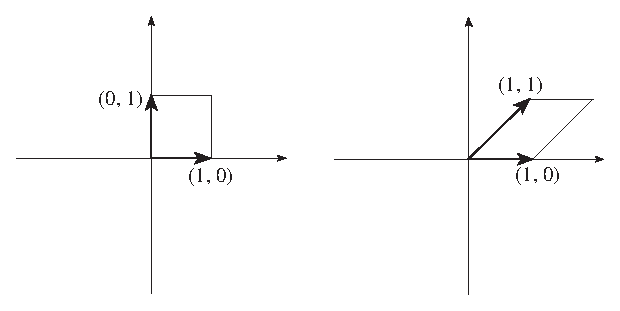
\includegraphics[width=2in]{SL2}
}
\end{center}
\caption{$SL_2({\Bbb R})$ acting on the unit square}
\label{SL2}
\end{figure}
 
 
 
\subsection*{The Orthogonal Group $O(n)$}
 
 
 
Another subgroup of $GL_n({\Bbb R})$ is the orthogonal group. A matrix
$A$ is {\bfi
orthogonal\/}\index{Orthogonal matrix}\index{Matrix!orthogonal} if
$A^{-1} = A^{\rm t}$. The {\bfi orthogonal
group\/}\index{Group!orthogonal}\index{Orthogonal group} consists of
the set of all orthogonal matrices. We write
$O(n)$\label{noteorthogonal} for the $n \times n$ orthogonal group. We
leave as an exercise the proof that $O(n)$ is a subgroup of $GL_n(
{\Bbb R})$.
 
 
\begin{example}{orthogonal}
The following matrices are orthogonal:
\[
\left(
\begin{array}{cc}
3/5 & -4/5 \\
4/5 & 3/5
\end{array}
\right), \; \;
\left(
\begin{array}{cc}
1/2 & -\sqrt{3}/2 \\
\sqrt{3}/2 & 1/2
\end{array}
\right), \; \;
\left(
\begin{array}{ccc}
-1/\sqrt{2} & 0 & 1/ \sqrt{2} \\
1/\sqrt{6} & -2/\sqrt{6} & 1/\sqrt{6} \\
1/ \sqrt{3} & 1/ \sqrt{3} & 1/ \sqrt{3} 
\end{array}
\right).
\]
\end{example}

 
There is a more geometric way of viewing the group $O(n)$. The
orthogonal matrices are exactly those matrices that preserve the
length of vectors. We can define the length of a vector using the
{\bfi Euclidean inner product},\index{Euclidean inner product} or
{\bfi dot product}, of two vectors. The Euclidean inner product of
two vectors ${\bold x}=(x_1, \ldots, x_n)^{\rm t}$ and ${\bold
y}=(y_1, \ldots, y_n)^{\rm t}$ is
\[
\langle  {\bold x}, {\bold y} \rangle
=
{\bold x}^{\rm t}  {\bold y}
=
(x_1, x_2, \ldots, x_n)
\left(
\begin{array}{c}
y_1 \\
y_2 \\
\vdots \\
y_n
\end{array}
\right)
=
x_1 y_1 + \cdots + x_n y_n.
\]
We define the length of a vector ${\bold x}=(x_1, \ldots, x_n)^{\rm
t}$ to be 
\[
\| {\bold x} \|\label{notelengthvect} 
= \sqrt{\langle  {\bold x}, {\bold x} \rangle} 
= \sqrt{x_1^2 + \cdots + x_n^2}.
\]
Associated with the notion of the length of a vector is the idea of
the distance between two vectors. We define the {\bfi distance\/}
between two vectors ${\bold x}$ and ${\bold y}$ to be $\| {\bold
x}-{\bold y} \|$. We leave as an exercise the proof of the following
proposition about the properties of Euclidean inner products.  
 
 
\begin{proposition}
Let ${\bold x}$, ${\bold y}$, and ${\bold w}$ be vectors in ${\Bbb
R}^n$ and $\alpha \in {\Bbb R}$. Then 
\begin{enumerate}
 
\rm \item \it
$\langle {\bold x}, {\bold y} \rangle = \langle {\bold y}, {\bold x}
\rangle$. 
 
\rm \item \it
$\langle {\bold x}, {\bold y} + {\bold w} \rangle = \langle {\bold x},
{\bold y} \rangle + \langle {\bold x}, {\bold w} \rangle$.
 
\rm \item \it
$\langle \alpha {\bold x}, {\bold y} \rangle = \langle {\bold x},
\alpha {\bold y} \rangle = \alpha \langle  {\bold x}, {\bold y}
\rangle$. 
 
\rm \item \it
$\langle {\bold x}, {\bold x} \rangle \geq 0$ with equality exactly
when ${\bold x} = 0$. 
 
\rm \item \it
If $\langle {\bold x}, {\bold y} \rangle = 0$  for all ${\bold x}$ in
${\Bbb R}^n$, then ${\bold y} = 0$. 
 
\end{enumerate}
\end{proposition}
 
 
\begin{example}{}
The vector ${\bold x} =(3,4)^{\rm t}$ has length $\sqrt{3^2 + 4^2} = 5$.  We
can also see that the orthogonal matrix 
\[
A=
\left(
\begin{array}{cc}
3/5 & -4/5 \\
4/5 & 3/5
\end{array}
\right)
\]
preserves the length of this vector. The vector $A{\bold x} =
(-7/5,24/5)^{\rm t}$ also has length 5. 
\end{example}
 
 
Since $\det(A A^{\rm t}) = \det(I) = 1$ and $\det(A) = \det( A^{\rm t}
)$, the determinant of any orthogonal matrix is either 1 or $-1$.
Consider the column vectors 
\[
{\bold a}_j
=
\left(
\begin{array}{c}
a_{1j} \\
a_{2j} \\
\vdots \\
a_{nj}
\end{array}
\right)
\]
of the orthogonal matrix
$A= (a_{ij})$. Since
$AA^{\rm t} = I$,
$\langle {\bold a}_r, {\bold a}_s \rangle = \delta_{rs}$,
where
\[
\delta_{rs}
=
\left\{
\begin{array}{cc}
1 & r = s \\
0 & r \neq s
\end{array}
\right.
\]
is the Kronecker delta\index{Kronecker delta}. Accordingly, column
vectors of an orthogonal matrix all have length 1; and the Euclidean
inner product of distinct column vectors is zero. Any set of vectors
satisfying these properties is called an {\bfi orthonormal
set}\index{Orthonormal set}. Conversely, given an $n \times n$ matrix
$A$ whose columns form an orthonormal set, $A^{-1} = A^{\rm t}$.
 
 
We say that a matrix $A$ is {\bfi
distance-preserving}\index{Matrix!distance-preserving}, {\bfi
length-preserving}\index{Matrix!length-preserving}, or {\bfi inner
product-preserving\/}\index{Matrix!inner product-preserving} when $\|
T{\bold x}- T{\bold y} \| =\| {\bold x}- {\bold y} \|$, $\| T{\bold x}
\| =\| {\bold x} \|$, or $\langle  T{\bold x}, T{\bold y} \rangle =
\langle {\bold x},{\bold y} \rangle$, respectively. The following
theorem, which characterizes the orthogonal group, says that these
notions are the same.
 
 
\begin{theorem}
Let $A$ be an $n \times n$ matrix.  The following statements are
equivalent. 
\begin{enumerate}
 
\rm \item \it
The columns of the matrix $A$ form an orthonormal set.
 
\rm \item \it
$A^{-1} = A^{\rm t}$.
 
\rm \item \it
For vectors ${\bold x}$ and ${\bold y}$, $\langle  A{\bold x}, A
{\bold y} \rangle = \langle  {\bold x}, {\bold y} \rangle$.
 
\rm \item \it
For vectors ${\bold x}$ and ${\bold y}$, $\| A{\bold x}- A{\bold y} \|
=\| {\bold x}- {\bold y} \|$. 
 
\rm \item \it
For any vector ${\bold x}$, $\| A{\bold x} \| = \| {\bold x}\|$.
 
\end{enumerate}
\end{theorem}
 
 
\begin{proof}
We have already shown (1) and (2) to be equivalent.
 
$(2) \Rightarrow (3)$.
\begin{eqnarray*}
\langle A{\bold x}, A{\bold y} \rangle
& = &
(A {\bold x})^{\rm t} A {\bold y} \\
& = &
{\bold x}^{\rm t} A^{\rm t} A {\bold y} \\
& = &
{\bold x}^{\rm t} {\bold y} \\
& = &
\langle {\bold x}, {\bold y} \rangle.
\end{eqnarray*}
 
$(3) \Rightarrow (2)$.
Since
\begin{eqnarray*}
\langle {\bold x}, {\bold x} \rangle
& = &
\langle A{\bold x}, A{\bold x} \rangle \\
& = &
{\bold x}^{\rm t} A^{\rm t} A {\bold y} \\
& = &
\langle {\bold x}, A^{\rm t} A{\bold x} \rangle,
\end{eqnarray*}
we know that $\langle {\bold x}, (A^{\rm t} A - I){\bold x} \rangle =
0$ for all ${\bold x}$.  Therefore, $A^{\rm t} A -I = 0$ or $A^{-1} =
A^{\rm t}$. 
 
 
$(3) \Rightarrow (4)$.
If $A$ is inner product-preserving, then $A$ is distance-preserving,
since 
\begin{eqnarray*}
\| A{\bold x} - A{\bold y} \|^2
& = &
\| A({\bold x} - {\bold y}) \|^2 \\
& = &
\langle
A({\bold x} - {\bold y}), A({\bold x} - {\bold y})
\rangle \\
& = &
\langle
{\bold x} - {\bold y}, {\bold x} - {\bold y}
\rangle \\
& = &
\| {\bold x} - {\bold y} \|^2.
\end{eqnarray*}
 
 
$(4) \Rightarrow (5)$.
If $A$ is distance-preserving, then $A$ is length-preserving. Letting
${\bold y} = 0$, we have
\[
\| A{\bold x}\|
= \| A{\bold x}- A{\bold y} \|
= \| {\bold x}- {\bold y} \|
= \| {\bold x} \|.
\]
 
 
$(5) \Rightarrow (3)$.
We use the following identity to show that length-preserving implies
inner product-preserving: 
\[
\langle {\bold x}, {\bold y} \rangle
=
\frac{1}{2}
\left[
\|{\bold x} +{\bold y}\|^2 -
 \|{\bold x}\|^2 - \|{\bold y}\|^2
\right].
\]
Observe that
\begin{eqnarray*}
\langle A {\bold x}, A {\bold y} \rangle
& = &
\frac{1}{2}
\left[
\|A {\bold x} + A {\bold y} \|^2
- \|A {\bold x} \|^2 -  \|A {\bold y} \|^2
\right] \\
& = &
\frac{1}{2}
\left[
\|A ( {\bold x} + {\bold y} ) \|^2
- \|A {\bold x} \|^2 -  \|A {\bold y} \|^2
\right] \\
& = &
\frac{1}{2}
\left[
\|{\bold x} + {\bold y}\|^2
- \|{\bold x}\|^2 - \|{\bold y}\|^2
\right] \\
& = &
\langle {\bold x}, {\bold y} \rangle.
\end{eqnarray*}
\end{proof}
 

 
 
\begin{figure}[htb]
\begin{center}
\centerline {
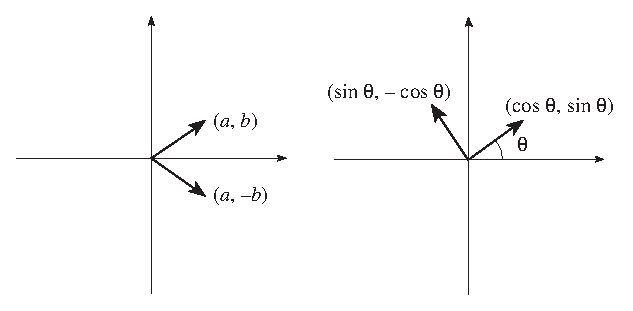
\includegraphics[width=2in]{O2}
}
\end{center}
\caption{$O(2)$ acting on ${\Bbb R}^2$}
\label{O2}
\end{figure}
 
\begin{example}{O2}
Let us examine the orthogonal group  on ${\Bbb R}^2$ a bit more
closely.  An element $T \in O(2)$ is determined by its action on
${\bold e}_1 = (1, 0)^{\rm t}$ and ${\bold e}_2 = (0, 1)^{\rm t}$. If
$T({\bold e}_1) = (a,b)^{\rm t}$, then $a^2 + b^2 = 1$ and $T({\bold
e}_2) = (-b, a)^{\rm t}$. Hence, $T$ can be represented by 
\[
A
=
\left(
\begin{array}{cc}
a & -b \\
b & a
\end{array}
\right)
=
\left(
\begin{array}{cc}
\cos \theta & - \sin \theta \\
\sin \theta & \cos \theta
\end{array}
\right),
\]
where $0 \leq \theta < 2 \pi$. A matrix $T$ in $O(2)$ either reflects
or rotates a vector in ${\Bbb R}^2$ (Figure~\ref{O2}). A reflection is
given by the matrix 
\[
\left(
\begin{array}{cc}
1 & 0 \\
0 & -1
\end{array}
\right),
\]
whereas a rotation by an angle $\theta$ in a counterclockwise direction
must come from a matrix of the form 
\[
\left(
\begin{array}{cc}
\cos \theta & \sin \theta \\
\sin \theta & -\cos \theta
\end{array}
\right).
\]
If $\det A =-1$, then $A$ gives a reflection.
\end{example}
 
 
 
Two of the other matrix or matrix-related groups that we will consider
are the special orthogonal group  and the group of Euclidean motions.
The {\bfi special orthogonal group}\index{Group!special orthogonal},
$SO(n)$\label{notespecialorthog}, is just the intersection of $O(n)$
and $SL_n({\Bbb R})$; that is, those elements in $O(n)$ with determinant
one. The {\bfi Euclidean
group}\index{Euclidean group}\index{Group!Euclidean},
$E(n)$\label{noteeuclidgroup}, can be written as ordered pairs $(A,
{\bold x})$, where $A$ is in $O(n)$ and ${\bold x}$ is in ${\Bbb
R}^n$. We define multiplication by
\[
(A, {\bold x}) (B, {\bold y})
=
(AB, A {\bold y} +{\bold x}).
\]
The identity of the group is $(I,{\bold 0})$; the inverse of $(A,
{\bold x})$ is $(A^{-1}, -A^{-1} {\bold x})$. In Exercise~6, you 
are asked to check that $E(n)$ is indeed a group under this operation.
 
 
 
 
\begin{figure}[hbt]
\begin{center}
\centerline {
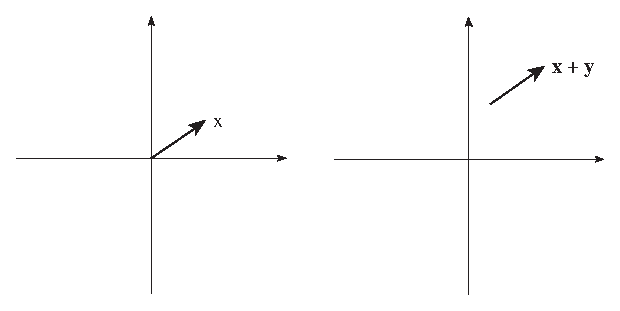
\includegraphics[width=2in]{Isometries}
}
\end{center}
\caption{Translations in ${\Bbb R}^2$}
\label{Isometries}
\end{figure}
 
 
 
 
 
\section{Symmetry}
 
 
 
 
An {\bfi isometry\/}\index{Isometry} or {\bfi rigid
motion\/}\index{Rigid motion} in ${\Bbb R}^n$  is a
distance-preserving function $f$ from ${\Bbb R}^n$ to ${\Bbb R}^n$.
This means that $f$ must satisfy 
\[
\| f({\bold x}) - f({\bold y}) \| =
\|{\bold x} - {\bold y} \|
\]
for all ${\bold x}, {\bold y} \in {\Bbb R}^n$. It is not difficult to
show that $f$ must be a one-to-one map. By Theorem~10.2, any element in
$O(n)$ is an isometry on ${\Bbb R}^n$; however, $O(n)$ does not
include all possible isometries on ${\Bbb R}^n$. Translation by a
vector ${\bold x}$, $T_{\bold y}({\bold x}) = {\bold x} + {\bold y}$
is also an isometry (Figure~\ref{Isometries}); however, $T$ cannot be
in $O(n)$ since it is not a linear map. 
 
 
 
We are mostly interested in isometries in ${\Bbb R}^2$. In fact, the
only isometries in ${\Bbb R}^2$ are rotations and reflections  about
the origin, translations, and combinations of the two. For example, a
{\bfi glide reflection\/}\index{Glide reflection} is a translation
followed by a reflection (Figure~\ref{Glide}).   In ${\Bbb R}^n$ all
isometries are given in the same manner. The proof is very easy to
generalize. 
 
 
\begin{figure}[htb]
\begin{center}
\centerline {
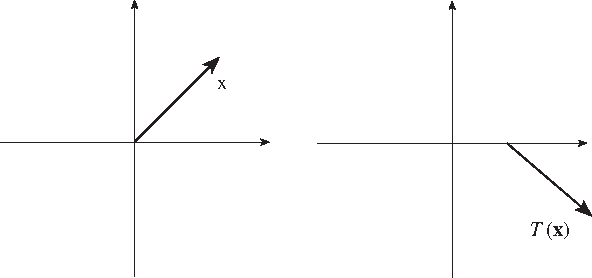
\includegraphics[width=2in]{Glide}
}
\end{center}
\caption{Glide reflections}
\label{Glide}
\end{figure}
 
 
\begin{lemma}
An isometry $f$ that fixes the origin in ${\Bbb R}^2$ is a linear
transformation.  In particular, $f$ is given by an element in $O(2)$. 
\end{lemma}
 
 
\begin{proof}
Let $f$ be an isometry in ${\Bbb R}^2$ fixing the origin. We will
first show that $f$ preserves inner products. Since $f(0) = 0$, $\|
f({\bold x})\| = \| {\bold x} \|$; therefore,
\begin{eqnarray*}
\| {\bold x} \|^2 - 2 \langle f({\bold x}), f({\bold y}) \rangle + \|
{\bold y} \|^2 
& = &
\| f({\bold x}) \|^2 - 2 \langle f({\bold x}), f({\bold y}) \rangle +
\| f({\bold y}) \|^2 \\ 
& = &
\langle
f({\bold x}) -  f({\bold y}), f({\bold x}) -  f({\bold y})
\rangle \\
& = &
\| f({\bold x}) -  f({\bold y}) \|^2 \\
& = &
\| {\bold x} -  {\bold y} \|^2 \\
& = &
\langle
{\bold x} -  {\bold y}, {\bold x} -  {\bold y} \rangle \\
& = &
\| {\bold x} \|^2 - 2 \langle {\bold x}, {\bold y} \rangle + \| {\bold
y} \|^2. 
\end{eqnarray*}
Consequently,
\[
\langle f({\bold x}), f({\bold y}) \rangle
=
\langle {\bold x}, {\bold y} \rangle.
\]
Now let ${\bold e}_1$ and ${\bold e_2}$ be $(1, 0)^{\rm t}$ and $(0,
1)^{\rm t}$, respectively. If 
\[
{\bold x} = (x_1, x_2) = x_1 {\bold e}_1 + x_2 {\bold e}_2,
\]
then
\[
f({\bold x})
=
\langle
f({\bold x}), f({\bold e}_1)
\rangle
f({\bold e}_1)
+\langle
f({\bold x}), f({\bold e}_2)
\rangle
f({\bold e}_2)
=
x_1 f({\bold e}_1)+x_2 f({\bold e}_2).
\]
The linearity of $f$ easily follows.
\end{proof}
 
 
\medskip
 
 
For any arbitrary isometry, $f$,  $T_{\bold x} f$ will fix the origin
for some vector ${\bold x}$ in ${\Bbb R}^2$; hence, $T_{\bold x}
f({\bold y}) = A {\bold y}$ for some matrix $A \in O(2)$.
Consequently, $f({\bold y}) = A {\bold y} + {\bold x}$.  Given the
isometries 
\begin{eqnarray*}
f({\bold y}) & = & A {\bold y} + {\bold x}_1 \\
g({\bold y}) & = & B {\bold y} + {\bold x}_2,
\end{eqnarray*}
their composition is
\[
f(g({\bold y})) =
f(B {\bold y} + {\bold x}_2) =
AB {\bold y} + A{\bold x}_2 + {\bold x}_1.
\]
This last computation allows us to identify the group of isometries on
${\Bbb R}^2$ with~$E(2)$. 
 
 
\begin{theorem}
The group of isometries on ${\Bbb R}^2$ is the Euclidean group,
$E(2)$. 
\end{theorem}
 
 
A {\bfi symmetry group\/}\index{Group!symmetry} in ${\Bbb R}^n$ is a
subgroup of the group of isometries on ${\Bbb R}^n$ that fixes a set
of points $X \subset {\Bbb R}^2$.  It is important to realize that the
symmetry group of $X$ depends {\em both\/} on ${\Bbb R}^n$ and on
$X$. For example, the symmetry group of the origin in ${\Bbb R}^1$ is
${\Bbb Z}_2$, but the symmetry group of the origin in ${\Bbb R}^2$ is
$O(2)$. 
 
 
\begin{theorem}
The only finite symmetry groups in ${\Bbb R}^2$ are ${\Bbb Z}_n$ and
$D_n$. 
\end{theorem}
 
 
\begin{proof}
Any finite symmetry group $G$ in ${\Bbb R}^2$ must be a finite
subgroup of $O(2)$; otherwise, $G$ would have an element in $E(2)$ of
the form $(A, {\bold x})$, where ${\bold x} \neq 0$.  Such an element
must have infinite order. 
 
 
By Example~6, elements in $O(2)$ are either rotations of the form
\[
R_{\theta}
=
\left(
\begin{array}{cc}
\cos \theta & - \sin \theta \\
\sin \theta & \cos \theta
\end{array}
\right)
\]
or reflections of the form
\[T_{\theta}
=
\left(
\begin{array}{cc}
\cos \theta & - \sin \theta \\
\sin \theta & \cos \theta
\end{array}
\right).
\]
Notice that $\det(R_{\theta})=1$,  $\det(T_{\theta})=-1$,
and $T_{\theta}^2=I$. We can divide the proof up into two cases.  In
the first case, all of the elements in $G$ have determinant one. In the
second case, there exists at least one element in $G$ with 
determinant~$-1$.  
 
 
{\em Case 1.}  
The determinant of every element in $G$ is one. In this case every
element in $G$ must be a rotation. Since $G$ is finite, there is a
smallest angle, say $\theta_0$, such that the corresponding element
$R_{\theta_0}$ is the smallest rotation in the positive direction.  We
claim that $R_{\theta_0}$ generates $G$.  If not, then for some
positive integer $n$ there is an angle $\theta_1$ between $n \theta_0$
and $(n+1) \theta_0$. If so, then $(n+1) \theta_0 - \theta_1$
corresponds to a rotation smaller than $\theta_0$, which contradicts
the minimality of $\theta_0$.   
 
 
 
{\em Case 2.}  
The group $G$ contains a reflection $T_{\theta}$.  The kernel of the
homomorphism $\phi : G \rightarrow \{-1, 1\}$ given by $A \mapsto
\det(A)$ consists of elements whose determinant is 1.  Therefore, $|G/
\ker \phi|=2$.  We know that the kernel is cyclic by the first case
and is a subgroup of $G$ of, say, order $n$. Hence, $|G| = 2n$. The
elements of $G$ are
\[
R_{\theta}, \ldots, R_{\theta}^{n-1},  TR_{\theta}, \ldots,
TR_{\theta}^{n-1}.
\]
These elements satisfy the relation
\[
TR_{\theta}T = R_{\theta}^{-1}.
\]
Consequently, $G$ must be isomorphic to $D_n$ in this case.
\end{proof}
 
 
 
 
\begin{figure}[thb]
\begin{center}
\centerline {
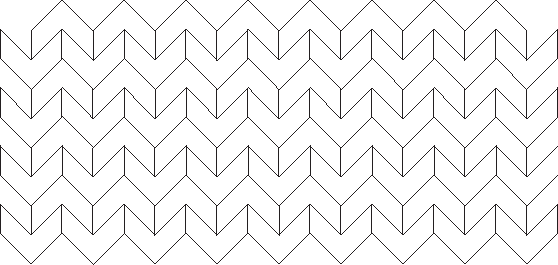
\includegraphics[width=2in]{Wallpaper}
}
\end{center}
\caption{A wallpaper pattern in ${\Bbb R}^2$}
\label{Wallpaper}
\end{figure}
 
 
 
\subsection*{The Wallpaper Groups}
 
 
 
Suppose that we wish to study wallpaper patterns in the plane or
crystals in three dimensions. Wallpaper patterns are simply repeating
patterns in the plane (Figure~\ref{Wallpaper}). The analogs of
wallpaper patterns in ${\Bbb R}^3$ are crystals, which we can think of
as repeating patterns of molecules in three dimensions
(Figure~\ref{Crystals}). The mathematical equivalent of a wallpaper or
crystal pattern is called a  lattice. 
 
 
 
\begin{figure}[hbt]
\begin{center}
\centerline {
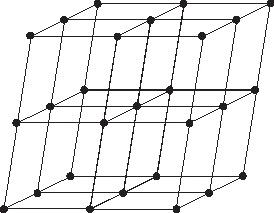
\includegraphics[width=2in]{Crystals}
}
\end{center}
\caption{A crystal structure in ${\Bbb R}^3$}
\label{Crystals}
\end{figure}
 
 

Let us examine wallpaper patterns in the plane a
little more closely. Suppose that ${\bold x}$ and ${\bold y}$ are
linearly independent vectors in ${\Bbb R}^2$; that is, one vector
cannot be a scalar multiple of the other. A {\bfi
lattice\/}\index{Lattice of points} of ${\bold x}$ and ${\bold y}$ is
the set of all linear combinations $m {\bold x} + n {\bold y}$, where
$m$ and $n$ are integers. The vectors ${\bold x}$ and ${\bold y}$ are
said to be a {\bfi basis\/}\index{Basis of a lattice} for the lattice.
 
 
\begin{figure}[htb]
\begin{center}
\centerline {
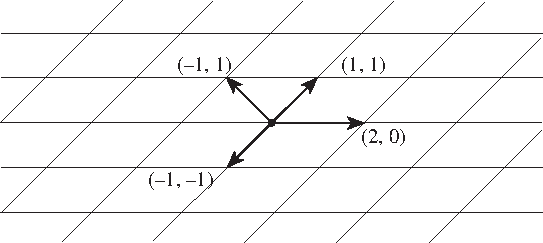
\includegraphics[width=2in]{LatticeExample}
}
\end{center}
\caption{A lattice in  ${\Bbb R}^2$}
\label{lattice}
\end{figure}
 
 
Notice that a lattice can have several bases. For example, the vectors
$(1,1)^{\rm t}$ and $(2,0)^{\rm t}$ have the  same lattice as the
vectors $(-1, 1)^{\rm t}$ and $(-1, -1)^{\rm t}$
(Figure~\ref{lattice}). However, any lattice is completely determined
by a basis. Given two bases for the same lattice, say $\{ {\bold x}_1,
{\bold x}_2 \}$ and $\{ {\bold y}_1, {\bold y}_2 \}$, we can write 
\begin{eqnarray*}
{\bold y}_1 & = & \alpha_1  {\bold x}_1 + \alpha_2 {\bold x}_2 \\
{\bold y}_2 & = & \beta_1  {\bold x}_1 + \beta_2 {\bold x}_2,
\end{eqnarray*}
where $\alpha_1$, $\alpha_2$, $\beta_1$, and $\beta_2$ are integers.
The matrix corresponding to this transformation is 
\[
U
=
\left(
\begin{array}{cc}
\alpha_1 & \alpha_2 \\
\beta_1 & \beta_2
\end {array}
\right).
\]
If we wish to give ${\bold x}_1$ and ${\bold x}_2$ in terms of ${\bold
y}_1$ and ${\bold y}_2$, we need only calculate $U^{-1}$; that is, 
\[
U^{-1}
\left(
\begin{array}{c}
{\bold y}_1 \\
{\bold y}_2
\end{array}
\right)
=
\left(
\begin{array}{c}
{\bold x}_1 \\
{\bold x}_2
\end{array}
\right).
\]
Since $U$ has integer entries, $U^{-1}$ must also have integer
entries; hence the determinants of both $U$ and $U^{-1}$ must be
integers. Because $U U^{-1} = I$,  
\[
\det(U U^{-1}) =\det(U) \det( U^{-1}) = 1;
\]
consequently, $\det(U) = \pm 1$. A matrix with determinant $\pm 1$ and
integer entries is called {\bfi unimodular}\index{Matrix!unimodular}.
For example, the matrix 
\[
\left(
\begin{array}{cc}
3 & 1 \\
5 & 2
\end{array}
\right)
\]
is unimodular. It should be clear that there is a minimum length for
vectors in a lattice.  
 
 
We can classify lattices by studying their symmetry groups. The
symmetry group of a lattice is the subgroup of $E(2)$ that maps the
lattice to itself. We consider two lattices in ${\Bbb R}^2$ to be
equivalent if they have the same symmetry group.  Similarly,
classification of crystals in ${\Bbb R}^3$ is accomplished by
associating a symmetry group, called a {\bfi space group}, with each
type of crystal\index{Group!space}. Two lattices are considered
different if their space groups are not the same.  The natural
question that now arises is how many space groups exist. 
 
 
A space group is composed of two parts: a {\bfi translation
subgroup\/}\index{Subgroup!translation} and a {\bfi point
group}\index{Group!point}.  The translation subgroup is an infinite
abelian subgroup of the space group made up of the translational
symmetries of the crystal; the point group is a finite group 
consisting  of rotations and reflections of the crystal about a point.
More specifically, a space group is a subgroup of $G \subset E(2)$
whose translations are a set of the form $\{ (I, t) : t \in L \}$,
where $L$ is a lattice. Space groups are, of course, infinite. Using
geometric arguments, we can prove the following theorem (see [5] or [6]).
 
 
 
 
\begin{theorem}
Every translation group in ${\Bbb R}^2$ is isomorphic to ${\Bbb Z}
\times {\Bbb Z}$.
\end{theorem}
 
 
\begin{figure}[bht]
\begin{center}
\centerline {
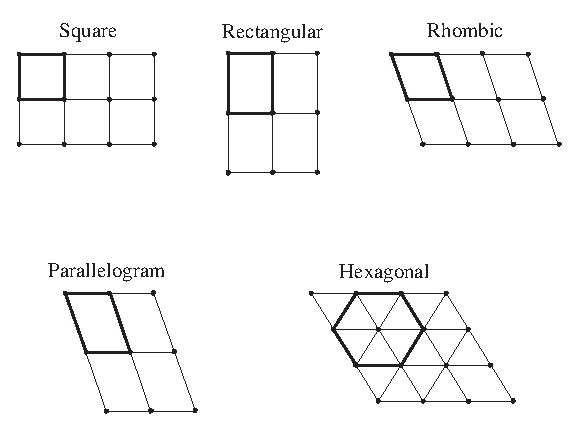
\includegraphics[width=2in]{TypeLattice}
}
\end{center}
\caption{Types of lattices in  ${\Bbb R}^2$}
\label{Types}
\end{figure}
 
 
The point group of $G$ is $G_0 = \{A : (A,b) \in G \mbox{ for some
$b$}  \}$. In particular, $G_0$ must be a subgroup of $O(2)$. Suppose
that ${\bold x}$ is a vector in a lattice $L$ with space group $G$,
translation group $H$, and point group $G_0$. For any element $(A,
{\bold y})$ in $G$,   
\begin{eqnarray*}
(A, {\bold y}) (I, {\bold x}) (A, {\bold y})^{-1}
& = &
(A,A {\bold x} + {\bold y}) (A^{-1},-A^{-1} {\bold y}) \\
& = &
(A A^{-1},-A A^{-1} {\bold y} + A {\bold x} + {\bold y}) \\
& = &
(I, A {\bold x});
\end{eqnarray*}
hence, $(I, A {\bold x})$ is in the translation group of $G$. More
specifically, $A {\bold x}$ must be in the lattice $L$. It is
important to note that $G_0$ is not usually a subgroup of the space
group $G$; however, if $T$ is the translation subgroup of $G$, then
$G/T \cong G_0$. The proof of the following theorem can be found in
[2], [5], or~[6].
 
 
 
\begin{theorem}
The point group in the wallpaper groups is isomorphic to ${\Bbb Z}_n$
or $D_n$, where $n = 1, 2, 3, 4, 6$. 
\end{theorem}
 
 
To answer the question of how the point groups and the translation
groups can be combined, we must look at the different types of
lattices. Lattices can be classified by the structure of a single
lattice cell. The possible cell shapes are parallelogram, rectangular,
square, rhombic, and hexagonal (Figure~\ref{Types}). The wallpaper
groups can now be classified according to the types of reflections
that occur in each group: these are ordinarily reflections, glide
reflections, both, or none.
 
 
 
\begin{table}[htb]
\caption{The 17 wallpaper groups}{\small
\begin{center}
\begin{tabular}{|l|l|l|l|}
\hline
Notation and &             &              & Reflections  \\
Space Groups & Point Group & Lattice Type & or Glide Reflections? \\
\hline
p1 & ${\Bbb Z}_1$ & parallelogram & none \\
p2 & ${\Bbb Z}_2$ & parallelogram & none \\
p3 & ${\Bbb Z}_3$ & hexagonal & none \\
p4 & ${\Bbb Z}_4$ & square & none \\
p6 & ${\Bbb Z}_6$ & hexagonal & none \\
pm & $D_1$ & rectangular & reflections \\
pg & $D_1$ & rectangular & glide reflections\\
cm & $D_1$ & rhombic & both \\
pmm & $D_2$ & rectangular & reflections \\
pmg & $D_2$ & rectangular & glide reflections \\
pgg & $D_2$ & rectangular & both \\
c2mm & $D_2$ & rhombic & both \\
p3m1, p31m & $D_3$ & hexagonal & both \\
p4m, p4g & $D_4$ & square & both \\
p6m & $D_6$ & hexagonal & both \\
\hline
\end{tabular}
\end{center}
}
\end{table}
 
 
\begin{theorem}
There are exactly 17 wallpaper groups.
\end{theorem}
 
 
\begin{figure}[htb]
\begin{center}
\centerline {
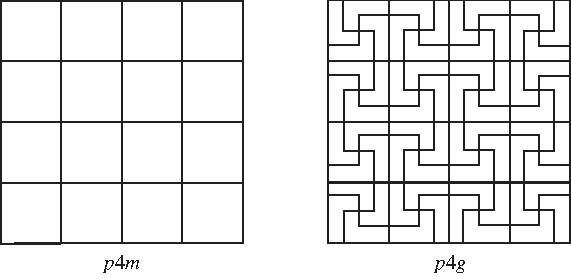
\includegraphics[width=2in]{p4m}
}
\end{center}
\caption{The wallpaper groups p4m and  p4g}
\label{p4m}
\end{figure}
 
 
 
The 17 wallpaper groups are listed in Table~10.1. The groups p3m1 and
p31m can be distinguished by whether or not all of their threefold
centers lie on the reflection axes: those of p3m1 must, whereas those
of p31m may not. Similarly, the fourfold centers of p4m must lie on
the reflection axes whereas those of p4g need not (Figure~\ref{p4m}).
The complete proof of this theorem can be found in several of the
references at the end of this chapter, including [5], [6], [10],
and~[11]. 
 
 
 
\histhead
 
 
\noindent{\small \histf
Symmetry groups have intrigued mathematicians for a long time.
Leonardo da Vinci was probably the first person to know all of the
point groups.  At the International Congress of Mathematicians in
1900, David Hilbert\index{Hilbert, David} gave a now-famous address
outlining 23 problems to guide mathematics in the twentieth
century.  Hilbert's eighteenth problem asked whether or not
crystallographic groups in $n$ dimensions were always finite.  In
1910, L.~Bieberbach\index{Bieberbach, L.} proved that crystallographic
groups are finite in every dimension.  Finding out how many of these
groups there are in each dimension is another matter. In ${\Bbb R}^3$
there are 230 different space groups; in ${\Bbb R}^4$ there are 4783.
No one has been able to compute the number of space groups for ${\Bbb
R}^5$ and beyond. It is interesting to note that the crystallographic
groups were found mathematically for ${\Bbb R}^3$ before the 230
different types of crystals were actually discovered in nature.
\histbox
}
 
 
 
\markright{EXERCISES}
\section*{Exercises}
\exrule
 
 
{\small
\begin{enumerate}
 
 
 
\bf\item\rm
Prove the identity
\[
\langle {\bold x}, {\bold y} \rangle = \frac{1}{2}
\left[
\|{\bold x} + {\bold y}\|^2 - \|{\bold x}\|^2 - \| {\bold y}\|^2
\right].
\]
 
 
\bf\item\rm
Show that $O(n)$ is a group.
 
 
\bf\item\rm
Prove that the following matrices are orthogonal. Are any of
these matrices in $SO(n)$?
 
\vspace{3pt}        %two column exercise list
 
\hspace{-7pt}
\begin{minipage}[t]{4.6in}
\noindent
\begin{minipage}[t]{2.25in}
\begin{itemize}
 
 \item[{\bf (a)}]
\raisebox{-5.5pt}{\parbox{1.85in}{
\[
\left(
\begin{array}{cc}
1/\sqrt{2} & -1/\sqrt{2} \\
1/\sqrt{2} & 1/\sqrt{2}
\end{array}
\right)
\]
}}

 
 \item[{\bf (c)}]
\raisebox{-11.5pt}{\parbox{1.85in}{
\[
\left(
\begin{array}{ccc}
4/ \sqrt{5} & 0 & 3 / \sqrt{5} \\
-3 / \sqrt{5} & 0 & 4 / \sqrt{5} \\
0 & -1 & 0
\end{array}
\right)
\] 
}}

\end{itemize}
\end{minipage} \hfill
\begin{minipage}[t]{2.25in}
\begin{itemize}
 
 \item[{\bf (b)}]
\raisebox{-5.5pt}{\parbox{1.85in}{
\[
\left(
\begin{array}{cc}
1 / \sqrt{5} & 2 / \sqrt{5} \\
- 2 /\sqrt{5} & 1/ \sqrt{5}
\end{array}
\right)
\]
}} 
 
 
 \item[{\bf (d)}]
\raisebox{-11.5pt}{\parbox{1.85in}{
\[
\left(
\begin{array}{ccc}
1/3 & 2/3 & - 2/3 \\
- 2/3 & 2/3 & 1/3 \\
-2/3 & 1/3 & 2/3
\end{array}
\right)
\]
}}
 
 
\end{itemize}
\end{minipage}
\end{minipage}
 
\vspace{2pt}        %end two column exercise list
 
 
 
\bf\item\rm %%%%%%%%%%%%%%%%%%%%%%
Determine the symmetry group of each of the figures in
Figure~\ref{Determine}. 
\begin{figure}[htb]
\begin{center}
\centerline {
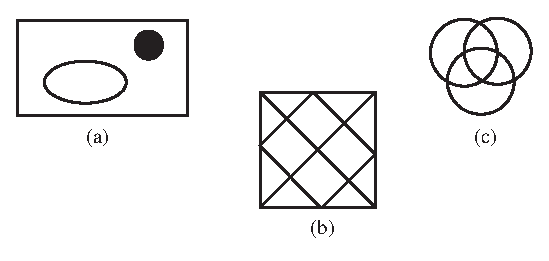
\includegraphics[width=2in]{SymmetryGrp}
}
\end{center}
\caption{}
\label{Determine}
\end{figure}
 
 
\bf\item\rm
Let ${\bold x}$, ${\bold y}$, and ${\bold w}$ be vectors in ${\Bbb
R}^n$ and $\alpha \in {\Bbb R}$.  Prove each of the following
properties of inner products.
\begin{enumerate}
 
 \bf\item\rm
$\langle {\bold x}, {\bold y} \rangle = \langle {\bold y}, {\bold x}
\rangle$. 
 
 \bf\item\rm
$\langle {\bold x}, {\bold y} + {\bold w} \rangle = \langle
{\bold x}, {\bold y} \rangle + \langle {\bold x}, {\bold w}
\rangle$.
 
 \bf\item\rm
$\langle \alpha {\bold x}, {\bold y} \rangle = \langle
{\bold x}, \alpha {\bold y} \rangle = \alpha \langle  {\bold
x}, {\bold y} \rangle$.
 
 \bf\item\rm
$\langle {\bold x}, {\bold x} \rangle \geq 0$ with equality exactly
when ${\bold x} = 0$. 
 
 \bf\item\rm
If $\langle {\bold x}, {\bold y} \rangle = 0$  for all ${\bold x}$ in
${\Bbb R}^n$, then ${\bold y} = 0$. 
 
\end{enumerate}
 
 
\bf\item\rm
Verify that
\[
E(n)
=
\{(A, {\bold x}) : A \in O(n) \mbox{ and } {\bold x} \in
{\Bbb R}^n \}
\]
is a group.
 
 
\bf\item\rm
Prove that $\{ (2,1), (1,1) \}$  and $\{ ( 12, 5), ( 7, 3) \}$ are bases
for the same lattice. 
 
 
\bf\item\rm
Let $G$ be a subgroup of $E(2)$ and suppose that $T$ is the
translation subgroup of $G$.  Prove that the point group of $G$ is
isomorphic to $G/T$. 
 
 
\bf\item\rm
Let $A \in SL_2({\Bbb R})$ and suppose that the vectors ${\bold x}$
and ${\bold y}$ form two sides of a parallelogram in ${\Bbb R}^2$.
Prove that the area of this parallelogram is the same as the area of
the parallelogram with sides $A{\bold x}$ and $A{\bold y}$. 
 
 
\bf\item\rm
Prove that $SO(n)$ is a normal subgroup of $O(n)$.
 
 
\bf\item\rm
Show that any isometry $f$ in ${\Bbb R}^n$ is a one-to-one map.
 
 
\bf\item\rm
Show that an element in $E(2)$ of the form $(A, {\bold x})$,
where ${\bold x} \neq 0$, has infinite order.
 
 
\bf\item\rm
Prove or disprove: There exists an infinite abelian subgroup of 
$O(n)$.
 
 
\bf\item\rm
Let ${\bold x} = (x_1, x_2)$ be a point on the unit circle in ${\Bbb
R}^2$; that is, $x_1^2 + x_2^2 = 1$. If $A \in O(2)$, show that $A
{\bold x}$ is also a point on the unit circle. 
 
 
 
\bf\item\rm
Let $G$ be a group with a subgroup $H$ (not necessarily normal) and a
normal subgroup $N$. Then $G$ is a {\bfi semidirect
product\/}\index{Semidirect product} of $N$ by $H$ if  
\begin{itemize}
 
 \item
$H \cap N = \{ id \}$;
 
 \item
$HN=G$.
 
\end{itemize}
Show that each of the following is true.
\begin{enumerate}
 
 \bf\item\rm
$S_3$ is the semidirect product of $A_3$ by $H = \{(1), (12) \}$.
 
 \bf\item\rm
The quaternion group, $Q_8$, cannot be written as a semidirect product. 
 
 \bf\item\rm
$E(2)$ is the semidirect product of $O(2)$ by $H$, where $H$ consists
of all translations in ${\Bbb R}^2$. 
 
\end{enumerate}
 
 
 
\bf\item\rm
Determine which of the 17 wallpaper groups preserves the symmetry of
the pattern in Figure~\ref{Wallpaper}.  
 
\begin{figure}[htb]
\begin{center}
\centerline {
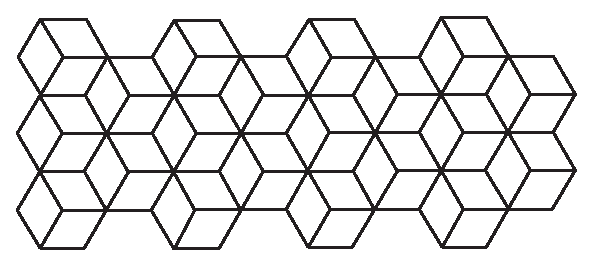
\includegraphics[width=2in]{p6m}
}
\end{center}
\caption{}
\label{For17}
\end{figure}
 
\bf\item\rm
Determine which of the 17 wallpaper groups preserves the symmetry of
the pattern in Figure~\ref{For17}.  
 
 
 
\bf\item\rm
Find the rotation group of a dodecahedron.
 
  
 
\bf\item\rm
For each of the 17 wallpaper groups, draw a wallpaper pattern having
that group as a symmetry group.  
 
\end{enumerate}
}
 
 
 
\subsection*{References and Suggested Readings}
 
 
 
{\small
\begin{itemize}
 
\item[{\bf [1]}]
Coxeter, H. M. and Moser, W. O. J. {\it Generators and
Relations for Discrete Groups}, 3rd ed. Springer-Verlag, New
York, 1972.
 
\item[{\bf [2]}]
Grove, L. C. and Benson, C. T. {\it Finite Reflection
Groups}. 2nd ed. Springer-Verlag, New York, 1985.
 
\item[{\bf [3]}]
Hiller, H. ``Crystallography and Cohomology of Groups,''
{\it American Mathematical Monthly} {\bf 93} (1986), 765--79.
 
\item[{\bf [4]}]
Lockwood, E. H. and Macmillan, R. H. {\it Geometric
Symmetry}. Cambridge University Press, Cambridge, 1978.
 
\item[{\bf [5]}]
Mackiw, G. {\it Applications of Abstract Algebra}. Wiley,
New York, 1985.
 
 
\item[{\bf [6]}]
Martin,  G.  {\it Transformation  Groups:  An Introduction to
Symmetry}.  Springer-Verlag, New York, 1982.
 
  
\item[{\bf [7]}]
Milnor, J. ``Hilbert's Problem 18: On Crystallographic
Groups, Fundamental Domains, and Sphere Packing,'' {\it
Proceedings of Symposia in Pure Mathematics} {\bf 18},
American Mathematical Society, 1976.
 
\item[{\bf [8]}]
Phillips, F. C. {\it An Introduction to Crystallography}.
4th ed. Wiley, New York, 1971.
 
\item[{\bf [9]}]
Rose, B. I. and Stafford, R. D. ``An Elementary Course in
Mathematical Symmetry,'' {\it American Mathematical Monthly} {\bf
88} (1980), 54--64.
 
 
\item[{\bf [10]}]
Schattschneider, D. ``The Plane Symmetry Groups: Their
Recognition and Their Notation,'' {\it American Mathematical 
Monthly} {\bf 85} (1978), 439--50.
 
 
\item[{\bf [11]}]
Schwarzenberger, R. L. ``The 17 Plane Symmetry Groups,'' {\it
Mathematical  Gazette} {\bf 58} (1974), 123--31. 
 
 
\item[{\bf [12]}]
Weyl, H. {\it Symmetry}. Princeton University Press, Princeton, NJ,
1952. 
 
 
\end{itemize}
}
 
 
 
 
